
\documentclass[12pt]{report}
\usepackage[utf8]{inputenc}

\usepackage{listings}
\usepackage{graphicx}
\usepackage{amsmath}
\usepackage{amsfonts}
\usepackage{amssymb}
\usepackage{pgfgantt}
\usepackage{amsthm}
\usepackage{fancyhdr}
\usepackage{rotating}
\usepackage[graphicx]{realboxes}
\renewcommand{\vec}{\bm}
\usepackage{dsfont}
\usepackage{xcolor}
\usepackage{sectsty}
\usepackage{tikz}
\usepackage{pgfplots}
\pgfplotsset{compat=newest}
\usepgfplotslibrary{patchplots}
\usetikzlibrary{calc,intersections,trees,positioning,arrows,chains,shapes.geometric,%
    decorations.pathreplacing,decorations.pathmorphing,shapes,%
    matrix,shapes.symbols, 3d}


\tikzset{
>=stealth',
  punktchain/.style={
    rectangle,
    rounded corners,
    % fill=black!10,
    draw=black, very thick,
    text width=10em,
    minimum height=3em,
    text centered,
    on chain},
  line/.style={draw, thick, <-},
  element/.style={
    tape,
    top color=white,
    bottom color=blue!50!black!60!,
    minimum width=8em,
    draw=blue!40!black!90, very thick,
    text width=10em,
    minimum height=3.5em,
    text centered,
    on chain},
  every join/.style={->, thick,shorten >=1pt},
  decoration={brace},
  tuborg/.style={decorate},
  tubnode/.style={midway, right=2pt},
  pics/carc/.style args={#1:#2:#3}{
    code={
      \draw[pic actions] (#1:#3) arc(#1:#2:#3);
    }
  }
}
% \usetikzlibrary{fadings}
\usepackage[paper=a4paper,top=0.58in,left=1.65in, right=1.65in, bottom=1.65in]{geometry}

\definecolor{lightorange}{RGB}{251,211,168}
\definecolor{darkred}{RGB}{153,0,0}
\definecolor{darkgreen}{RGB}{0,51,25}

% \sectionfont{\fontsize{12}{15}\selectfont}

\title{ \includegraphics[width=\linewidth]{header.png}~
\\[0.5cm]
  \huge{Bachelor Project} \\
\textbf{\Large{Barycentric Data Visualization for Triangle Meshes}}}
\date{Spring Semester 2018}
\author{Costanza \textbf{Volpini} \\ \textcolor{gray}{costanza.volpini@usi.ch} \\ \\ Professor: Kai \textbf{Hormann} \\ Assistant: Jan \textbf{Svoboda}}

\begin{document}
\pagestyle{fancy}
\rhead{\bfseries  Costanza Volpini}
\lhead{\bfseries  Project Proposal}
\maketitle
\newgeometry{paper=a4paper,margin=1.65in}

%%%%%%% ref: https://it.sharelatex.com/blog/2013/08/02/thesis-series-pt1.html
\chapter*{Abstract}
Abstract goes here

\chapter*{Dedication}
to somebody

\chapter*{Declaration}
I declare that..

\chapter*{Acknowledgements}
I want to thank...

\tableofcontents
%%%%%%%
\chapter{Introduction}
\section{Barycentric coordinates}
Let us consider a triangle with top, bottom left and bottom right vertices to which we have assigned the colors red, green and blue respectively. The triangle barycentre divides each median into two parts that have a 2:1 ratio. \\
  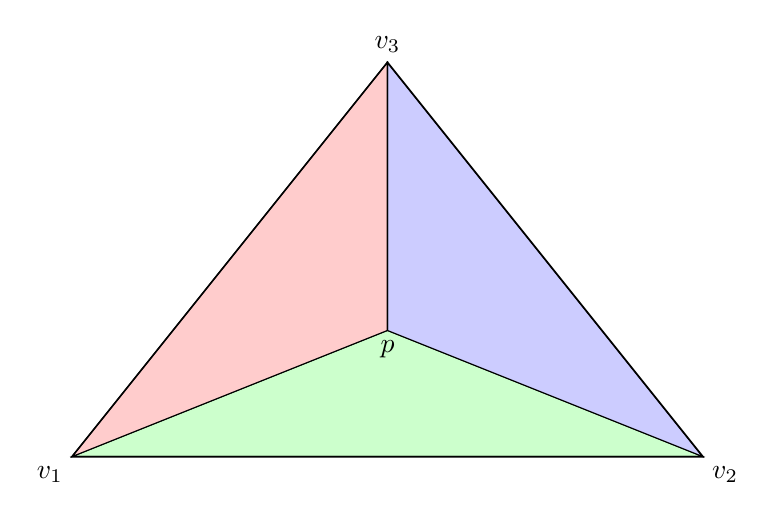
\begin{tikzpicture}
    \coordinate (L1) at (0,0);
    \coordinate (L2) at (8,0);
    \coordinate (L3) at (4,5);
    \coordinate (X) at (4,1.6);

    \draw[thick] (L1) -- coordinate[midway](md3) (L2)
                      -- coordinate[midway](md1) (L3)
                      -- coordinate[midway](md2) (L1) -- cycle;
    \filldraw[draw=black, fill=green!20] (L1) -- (X) -- (L2) -- cycle;
    \filldraw[draw=black, fill=red!20] (L1) -- (X) -- (L3) -- cycle;
    \filldraw[draw=black, fill=blue!20] (L3) -- (X) -- (L2) -- cycle;
    \draw (L1) node [below left] {$v_1$}
       -- (L2) node [below right] {$v_2$}
       -- (L3) node [above] {$v_3$}
       -- (X) node [below] {$p$};
    \end{tikzpicture}
    \\
    Let call the red area $w_1$, the blue green one $w_2$ and the blue one $w_3$. Normalazing each of them by the area of the triangle, we will get three values ($\lambda_1, \lambda_2, \lambda_3$) that are the barycentric coordinates of $p$ with respect to the triangle [$v_1, v_2, v_3$].
\\ \\ WRITE!!!!!!! introduction and all properties

\section{Linear Interpolation}
The standard linear interpolated visualisation is made passing three attributes (colors) for each vertex of a triangle. OpenGL will interpolate linearly the colors. That is possible thanks to the barycentric coordinates that will tell how much of each color is being mixed at any position.

\section{Flat Shading}

\section{Gouraud Shading}

\section{Gaussian Curvature}
\textit{Gaussian Curvature} works like a logical \texttt{AND}, it will check if there is a curvature along both directions.

\begin{figure}[h]
  \minipage[b]{.5\linewidth}
  \centering
  \scalebox{0.7}{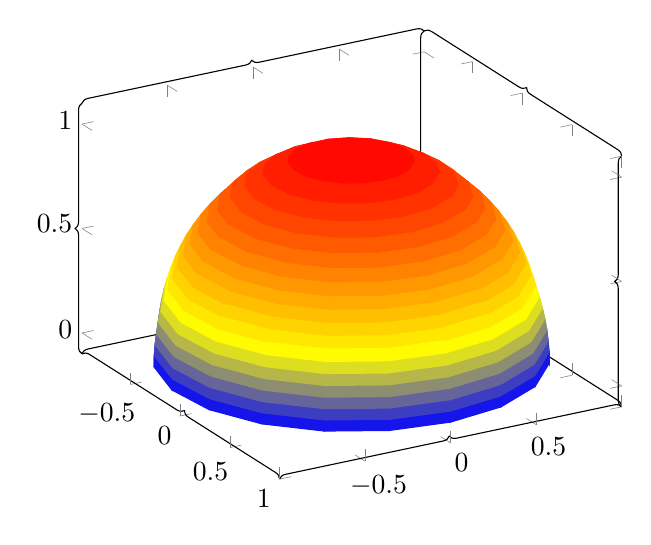
\begin{tikzpicture}
  \begin{axis}[view={60}{30}]
      \addplot3[surf,shader=flat,
          samples=20,
          domain=1:0,y domain=0:2*pi,
          z buffer=sort]
          ({sqrt(1-x^2) * cos(deg(y))},
       {sqrt( 1-x^2 ) * sin(deg(y))},
       x);
  \end{axis}
  \end{tikzpicture}}
  \caption{Positive gaussian curvature}\label{fig:positive-gaussian}
  \endminipage
  \minipage[b]{.5\linewidth}
  \centering
  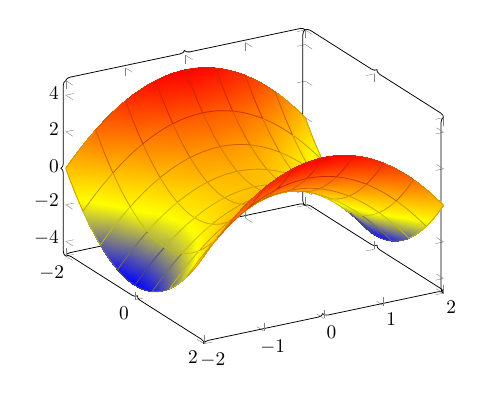
\begin{tikzpicture}[scale=0.7]
    \begin{axis}[view={60}{30}]
    \addplot3[patch,patch refines=3,
    shader=faceted interp,
    patch type=biquadratic]
    table[z expr=x^2-y^2]
    {
        x  y
        -2 -2
        2  -2
        2  2
        -2 2
        0  -2
        2  0
        0  2
        -2 0
        0  0
    };
  \end{axis}
  \end{tikzpicture}
  \endminipage
  \caption{Negative gaussian curvature}\label{fig:negative-gaussian}
\end{figure}


\chapter{GPU program}
shaders (geometry, vertex, fragment) + model view etc.
arcball/trackball

Shader program is written in \textit{GLSL}.

Vertex shader is done on every vertex (before rasterization).
Fragment shader is done on every pixel (coloring per fragment).

%%%%%%%%%
A program that runs on GPU is called \textit{shader}. Shaders are principally used to modify the representation and the behaviour of 3D objects. They are also used to create lighting effects.  Shaders can perform tasks efficiently thanks to the GPU. That guarantee faster results than CPU since GPU is designed to work in parallel.

\section{GPU pipeline}
% \\
% \\
\scalebox{0.85}{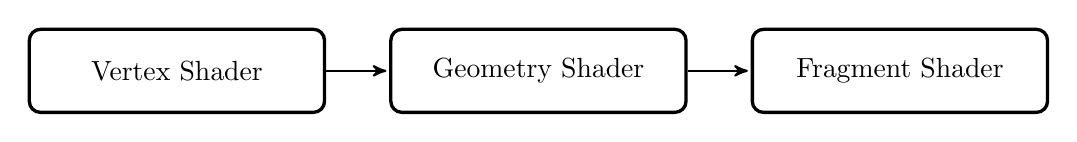
\begin{tikzpicture}
    [node distance=.8cm,
    start chain=going right,]
       \node[punktchain, join] (vs) {Vertex Shader};
       \node[punktchain, join] (gs)  {Geometry Shader};
       \node[punktchain, join] (fs)  {Fragment Shader};
\end{tikzpicture}}


\section{Vertex Shader}
The program that perform vertex operations is called \textit{vertex shader}. It receives one vertex at a time and then it passes the output to a \textit{fragment shader} or to a \textit{geometry shader}, if any.

\section{Fragment Shader}
\textit{Fragment shader} performs color computation for every visible pixel of the rasterized object. It works on a fragment at a time, but thanks to the power of GPU it can work in parallel for all vertices (\textit{vertex shader}) and fragments (\textit{fragment shader}).

\section{Geometry Shader}
\textit{Geometry shader} is used for layered rendering. It takes as input a set of vertices (single primitive, example: triangle or a point) and it transforms them before sending to the next shader stage. In this way, we can obtain different primitives.

Each time we call the function \texttt{EmitVertex()} the vector currently set to \texttt{gl\_Position} is added to the primitive. All emitted vertices are combined for the primitive and output when we call the function \texttt{EndPrimitive()}.
\\
\\
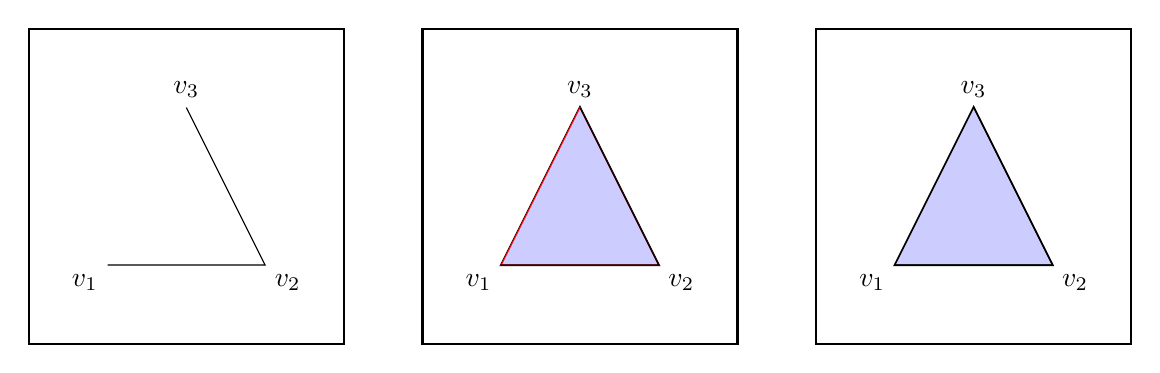
\begin{tikzpicture}
    \coordinate (L1) at (6,0);
    \coordinate (L2) at (8,0);
    \coordinate (L3) at (7,2);

    \coordinate (S1) at (5,-1);
    \coordinate (S2) at (9,-1);
    \coordinate (S3) at (5,3);
    \coordinate (S4) at (9,3);


    % \draw[thick] (L1) -- (L2)
    %                   -- (L3)
    %                   -- (L1) -- cycle;


    \draw[thick] (S1) --  (S2)
                      --  (S4)
                      --  (S3)
                      --  (S1) -- cycle;



    \coordinate (L11) at (11,0);
    \coordinate (L12) at (13,0);
    \coordinate (L13) at (12,2);

    \coordinate (S11) at (10,-1);
    \coordinate (S12) at (14,-1);
    \coordinate (S13) at (10,3);
    \coordinate (S14) at (14,3);


    \draw[thick] (L11) -- (L12)
                      -- (L13)
                      -- (L11) -- cycle;

    \draw[thick] (S11) --  (S12)
                      --  (S14)
                      --  (S13)
                      --  (S11) -- cycle;

    %%%
    \coordinate (L21) at (16,0);
    \coordinate (L22) at (18,0);
    \coordinate (L23) at (17,2);

    \coordinate (S21) at (15,-1);
    \coordinate (S22) at (19,-1);
    \coordinate (S23) at (15,3);
    \coordinate (S24) at (19,3);


    \draw[thick] (L21) -- (L22)
                      -- (L23)
                      -- (L21) -- cycle;

    \draw[thick] (S21) --  (S22)
                      --  (S24)
                      --  (S23)
                      --  (S21) -- cycle;
    % \filldraw[draw=black, fill=green!20] (L1) -- (X) -- (L2) -- cycle;
    % \filldraw[draw=black, fill=red!20] (L1) -- (X) -- (L3) -- cycle;
    \filldraw[draw=red, fill=blue!20] (L11) -- (L12) -- (L13) -- cycle;
    \filldraw[draw=black, fill=blue!20] (L21) -- (L22) -- (L23) -- cycle;
    \draw (L1) node [below left] {$v_1$}
       -- (L2) node [below right] {$v_2$}
       -- (L3) node [above] {$v_3$};

    \draw (L11) node [below left] {$v_1$}
       -- (L12) node [below right] {$v_2$}
       -- (L13) node [above] {$v_3$};

    \draw (L21) node [below left] {$v_1$}
       -- (L22) node [below right] {$v_2$}
       -- (L23) node [above] {$v_3$};
    \end{tikzpicture}

\chapter{Flat shading extension}
Alternative data visualization techniques can be found using the power of barycentric coordinates and GPU programming.

The usual way to visualize data for a triangle mesh is to associate data to vertices and then interpolating over the mesh triangles, that does not work in case of edges and triangles.

\section{Region around a vertex}
We can split the surface of triangle meshes into regions around vertex (Fig. \ref{fig:vertex-area}) and color them.

These regions can be determined using barycentric coordinates and GPU fragment program. Visualizing data given at the vertices or edges of the mesh in a piecewise constant simulates the classical triangle flat shading.
An example of this vertex data is the discrete Gaussian curvature.
\begin{figure}[h]
    \centering
    \minipage[b]{.5\linewidth}
    \centering
    \includegraphics[scale=0.2]{images/max.png}
    \caption{Vertex based area}\label{fig:max-diagram}
    \endminipage
    \minipage[b]{.5\linewidth}
    \centering
    \includegraphics[scale=0.2]{images/vertex-area.png}
    \caption{Region around a vertex}\label{fig:vertex-area}
    \endminipage
\end{figure}


\section{Max diagram - Vertex based area}
Passing barycentric coordinates to the fragment shader will clearly demonstrate that we can get results different from the classic color interpolation.

There are different approaches to color interpolation focusing on the distance from vertices. For each point in a triangle, we can easily determine its closest vertex, which we use as a cue for coloring.

A different approach from interpolating, can be found coloring vertex areas based on the minimum barycentric coordinate.
The color is given by the region farthest from a vertex (Fig. \ref{fig:max-diagram}).

\begin{lstlisting}[language=C++,
    directivestyle={\color{black}}
    emph={int,char,double,float,unsigned},
    emphstyle={\color{blue}}
   ]
if (Coords.x > Coords.y && Coords.x > Coords.z) {
    vec3 blue = vec3(0.0f, 0.0f, 1.0f);
    FragColor = vec4(blue, 1.0f);
} else if(Coords.y > Coords.x && Coords.y > Coords.z) {
    vec3 green = vec3(0.0f, 1.0f, 0.0f);
    FragColor = vec4(green, 1.0f);
} else {
    vec3 red = vec3(1.0f, 0.0f, 0.0f);
    FragColor = vec4(red, 1.0f);
}
\end{lstlisting}

\section{Implementation}
Suppose now that you want each vertex area to be in one constant color. This color can be taken from shading interpolation using the normal at the vertex and the vertex position. Then you can compute the color has it be done in \textit{Gouraud Shading}.

The idea is to compute the color per vertex but instead of linearly interpolated it in each triangle (as \textit{Gouraud shading} does) we color regions around a vertex with that constant color.

To implement that we need to pass the barycentric coordinates, the vertex color, the normal at the vertex and the lighting calculations to the \textit{fragment shader}.

We want to avoid an automatic interpolation of colors, in order to return the resulting color using the \textit{max diagram}, to do that we have used a \textit{Geometry shader} in order to access to all three vertex colors in fragment shader.
\\
\\
\scalebox{0.85}{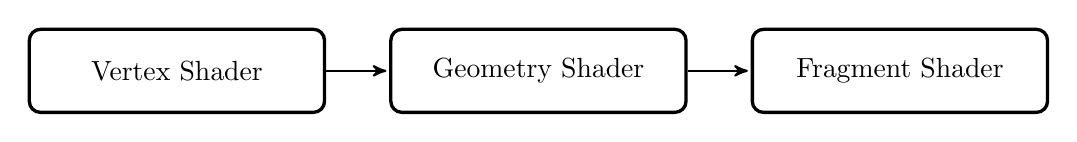
\begin{tikzpicture}
    [node distance=.8cm,
    start chain=going right,]
       \node[punktchain, join] (vs) {Vertex Shader};
       \node[punktchain, join] (gs)  {Geometry Shader};
       \node[punktchain, join] (fs)  {Fragment Shader};
\end{tikzpicture}}


% \subsection{Min diagram - Edge based area}
% A different approach from interpolating, can be found coloring edge areas based on the minimum barycentric coordinate.
% The color is given by the region closest to the vertex.

% \chapter{Conclusion}
% Making computation per vertex (e.g. \textit{Flat Shading}) is more efficient because in general, a model has fewer vertices than triangles as shown in table \ref{table:model-table-vertices}.
For example, the armadillo model has $15002$ vertices and $30000$ triangles, then make calculation per vertex instead of triangle results in half of the computations.

\begin{table}[!h]
    \centering
\begin{tabular}{l*{6}{c}r}
    \centering
    Model              & \#vertices & \#triangles & Improvement\\
    \hline
    Armadillo          & 15002 & 30000 & 49\%\\
    Eight              & 766 & 1536 & 50\% \\
    Genus3             & 6652 & 13312 & 50\% \\
    Horse              & 48485 &  96966 & 49\%\\
    Icosahedron\_1      &  42 & 80 & 47\%\\
    Icosahedron\_2      &  162 & 320 & 49\% \\
    Icosahedron\_3      & 642 &  1280 & 50\%
\end{tabular}
\caption{Number of vertices and triangles in models. Making computations per vertex result in an efficiency improvement of $\approx$ 50\%.}
\label{table:model-table-vertices}
\end{table}

Making computation per edge would also be more efficient, because edges are shared between $2$ triangles in a mesh.

\subsection{Application Software}
I have developed an application for alternative data visualization using the power of barycentric coordinates and GPU programming.
\begin{figure}[!h]
    \includegraphics[scale=0.4]{images/program.png}
    \caption{Software}
    \label{fig:software}
\end{figure}
This application allows the user to upload different models, choose different shaders, zoom or rotate the model.
In Fig. \ref{fig:software}, a \textit{constant Gaussian curvature} shader is chosen for a model using a $90 \; percentile$, on the right graphs plot Gaussian curvature values obtained for each vertex. The first graph shows the real values of Gaussian curvature without removing the outliers. The second graph shows just the values in the $90 \; percentile$ (all the outliers were discarded).

\subsection{Architecture}
The application was developed in c++, for the real-time graphics programming (e.g. create the scene viewer, enabling the manipulation of 3D scenes) I have used OpenGL $3.3$ and GLSL.

As graphical user interface I have used a library called \textit{Dear ImGui}. This library has no external dependencies and it is designed to create content creation tools and visualization/debug tools. It is suited to integration in games engine (for tooling), real-time 3D applications or any applications on console platforms where operating system features are non-standard.

To allow the creation of an OpenGL context, the definition of window parameters and to handle user inputs I have used the \textit{GLFW3} library.

Since there are different versions of OpenGL drivers, to retrieve the location of the functions required and to store them in function pointers for later use, I have used \textit{GLAD} library that loads all relevant OpenGL functions according to that version at compile-time.

\subsection{Comparison with meshlab}
All the values obtained for the \textit{Gouraud Gaussian curvature} and \textit{Gouraud mean curvature} were compared to the results provided by the program \textit{meshlab}\footnote{Meshlab is an open source system for processing and editing 3D triangular meshes.
It provides a set of tools for editing, cleaning, healing, inspecting, rendering, texturing and converting meshes. It offers features for processing raw data produced by 3D digitization tools/devices and for preparing models for 3D printing. \url{http://www.meshlab.net/}}.


\begin{table}[!h]%gauss
    \centering
\begin{tabular}{l*{6}{c}r}
    \centering
    Model              & our software &  meshlab   & absolute difference\\
    \hline
    Armadillo          & [-33034.20, 90017.90] & [-33033.84, 90019.63] & [0.36, 1.73] \\
    Eight              & [-116.89, 58.33] & [-116.89, 58.33] & [0.00, 0.00] \\
    Genus3             & [-1753.20, 209.18] & [-1753.20, 209.18] & [0.00, 0.00]  \\
    Horse              & [-321731, 1930410] &  [-4177.14, 4853.23] & [317553.86 1925556.77]\\
    Icosahedron\_1      &  [1.07, 1.08] & [1.07, 1.08] & [0.00, 0.00] \\
    Icosahedron\_2      &  [1.01, 1.02] & [1.01, 1.02] & [0.00, 0.00] \\
    Icosahedron\_3      & [1.00, 1.00] &  [1.00, 1.00] & [0.00, 0.00]
\end{tabular}
\caption{Our Gouraud Gaussian curvature values ([min, max]) and meshlab Gouraud Gaussian curvature values ([min, max]).}
\label{table:table-gaussian-meshlab}
\end{table}



\begin{table}[!h]%mean
    \centering
\begin{tabular}{l*{6}{c}r}
    \centering
    Model              & our software &  meshlab  & absolute difference\\
    \hline
    Armadillo          & [-289.74, 392.54] & [-289.74, 392.54] & [0.00, 0.00]\\
    Eight              & [1.35, 10.96] & [1.35, 10.96] & [0.00, 0.00]\\
    Genus3             & [-7.02, 117.34] & [-7.03, 117.34] & [0.00, 0.00] \\
    Horse              & [-500.96, 1202.51] &  [-500.96, 1202.51] & [0.00, 0.00]\\
    Icosahedron\_1      &  [0.10, 1.00] & [0.10, 1.00] & [0.00, 0.00]\\
    Icosahedron\_2      &  [0.10, 1.00] & [0.10, 1.00]& [0.00, 0.00] \\
    Icosahedron\_3      & [0.10, 1.00] &  [0.10, 1.00] & [0.00, 0.00]
\end{tabular}
\caption{Our Gouraud mean curvature values ([min, max]) and meshlab Gouraud mean curvature values ([min, max]).}
\label{table:table-mean-meshlab}
\end{table}




\appendix
\chapter{Appendix Title}
% \input{chapters/appendix}

\section{Extend Flat Shading}

% \section{Evaluation and comparison}
% \begin{figure}[!htb]
  % \minipage{0.32\textwidth}
  %   \includegraphics[width=\linewidth]{interpolation.png}
  %   \caption{Interpolation.}\label{fig:interpolation}
  % \endminipage\hfill
  % \minipage{0.32\textwidth}
  %   \includegraphics[width=\linewidth]{flat.png}
  %   \caption{Min Diagram.}\label{fig:min}
  % \endminipage\hfill
  % \minipage{0.32\textwidth}%
  %   \includegraphics[width=\linewidth]{gaussian.png}
  %   \caption{Gaussian Curvature}\label{fig:gaussian-horse}
  % \endminipage
  % \end{figure}

\end{document}

